\documentclass[12pt,twoside,a4paper]{article}
\usepackage[a4paper,width=150mm,top=25mm,bottom=25mm,bindingoffset=6mm]{geometry}

\usepackage[utf8x]{inputenc}
\usepackage[slovak]{babel}
\usepackage{palatino,verbatim}

% Balicek pre priamu rec - \say
\usepackage{dirtytalk}

% Obrazky
\usepackage{graphicx}
\graphicspath{ {obr/} }

% Cislovanie obrazkov a tabuliek
\usepackage{chngcntr}
%Cisluj obrazky nezavisle od cisla kapitol/podkapitol
%\counterwithout{figure}{subsection}
%\counterwithout{table}{subsection}

%Uloz obrazok tam, kde je deklarovany
%\usepackage[subsection]{placeins}

\newcommand\sktxt[1]{\foreignlanguage{slovak}{#1}}

\begin{document}
\pagenumbering{arabic}

\section*{Multi-area OSPF}
\subsection*{Topológia}
\paragraph{}
Budeme konfigurovať Multi-area OSPF, ktorá je znázornená na obrázku ~\ref{fig:multiarea_ospf_topo}.

\begin{figure}[!htb]
\centering
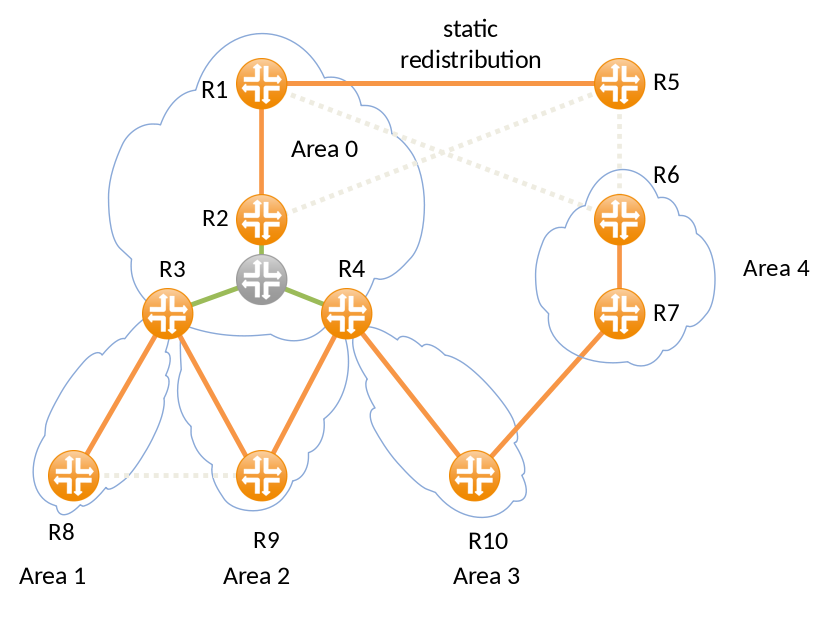
\includegraphics[width=12cm,keepaspectratio]{multiarea_ospf_topo}
\caption{Topológia Multi-area OSPF}
\label{fig:multiarea_ospf_topo}
\end{figure}

\subsection*{Úlohy a ich konfigurácia}
\subsubsection*{Základná konfigurácia}
\subparagraph{Popis}
\subparagraph{}
Ako za základnú konfiguráciu považujeme nastavenie adresácie, vzdialeného prístupu a vypisovania konzoly.
\subparagraph{Konfigurácia}
\noindent
{\fontfamily{qcr}\selectfont
\begin{small}
\begin{verbatim}
!!!!!!!!!!   R1   !!!!!!!!!!
hostname R1
no ip domain-lookup
username admin privilege 15 secret admin
line con 0
	login local
	logging synchronous
	exec-timeout 120
line vty 0 15
	privilege level 15
	no login
int lo1
	ip address 10.255.255.1 255.255.255.255
	no shutdown
int f0/1
	ip address 10.100.15.1 255.255.255.0
	no shutdown
int f0/0
	ip address 10.0.12.1 255.255.255.0
	no shutdown

do show ip interface brief


!!!!!!!!!!   R2   !!!!!!!!!!
hostname R2
no ip domain-lookup
username admin privilege 15 secret admin
line con 0
	login local
	logging synchronous
	! Predĺženie intervalu na odpojenie používateľa od konzoly
	exec-timeout 120
line vty 0 15
	privilege level 15
	no login
int lo1
	ip address 10.255.255.2 255.255.255.255
	no shutdown
int f0/1
	ip address 10.0.234.2 255.255.255.0
	no shutdown
int f0/0
	ip address 10.0.12.2 255.255.255.0
	no shutdown

do show ip interface brief


!!!!!!!!!!   R3   !!!!!!!!!!
hostname R3
no ip domain-lookup
username admin privilege 15 secret admin
line con 0
	login local
	logging synchronous
	exec-timeout 120
line vty 0 15
	privilege level 15
	no login
int lo1
	ip address 10.255.255.3 255.255.255.255
	no shutdown
int f0/1
	ip address 10.0.234.3 255.255.255.0
	no shutdown
int f0/0
	ip address 10.1.38.1 255.255.255.0
	no shutdown
int s1/0
	ip address 10.2.39.1 255.255.255.252
	no shutdown

do show ip interface brief


!!!!!!!!!!   R4   !!!!!!!!!!
hostname R4
no ip domain-lookup
username admin privilege 15 secret admin
line con 0
	login local
	logging synchronous
	exec-timeout 120
line vty 0 15
	privilege level 15
	no login
int lo1
	ip address 10.255.255.4 255.255.255.255
	no shutdown
int f0/1
	ip address 10.0.234.4 255.255.255.0
	no shutdown
int f0/0
	ip address 10.2.49.1 255.255.255.0
	no shutdown
int s1/0
	ip address 10.3.104.1 255.255.255.252
	no shutdown

do show ip interface brief


!!!!!!!!!!   R5   !!!!!!!!!!
hostname R5
no ip domain-lookup
username admin privilege 15 secret admin
line con 0
	login local
	logging synchronous
	exec-timeout 120
line vty 0 15
	privilege level 15
	no login
int lo1
	ip address 10.255.255.5 255.255.255.255
	no shutdown
int f0/1
	ip address 10.100.15.2 255.255.255.0
	no shutdown

do show ip interface brief

!!!!!!!!!!   R6   !!!!!!!!!!
hostname R6
no ip domain lookup
username admin privil 15 secret admin
line con 0
	login local
	logging synchro
	exec-timeout 120
line vty 0 15
	privilege level 15	
	no login
int lo1
	ip add 10.255.255.6 255.255.255.255
	no sh
int fa0/1 
	ip add 10.4.67.1 255.255.255.0
	no sh

!!!!!!!!!!   R7   !!!!!!!!!!
hostname R7
no ip domain lookup
username admin privil 15 secret admin
line con 0
	login local
	logging synchro
	exec-timeout 120
line vty 0 15
	privilege level 15	
	no login
int lo1
	ip add 10.255.255.7 255.255.255.255
	no sh
int fa0/1 
	ip add 10.4.67.2 255.255.255.0
	no sh
int s1/1
	ip add 10.4.107.1 255.255.255.0
	no sh

!!!!!!!!!!   R8   !!!!!!!!!!
hostname R8
no ip domain lookup
username admin privil 15 secret admin
line con 0
	login local
	logging synchro
	exec-timeout 120
line vty 0 15
	privilege level 15	
	no login
int lo1
	ip add 10.255.255.8 255.255.255.255
	no sh
int fa0/0 
	ip add 10.1.38.2 255.255.255.0
	no sh

!!!!!!!!!!   R9   !!!!!!!!!!
hostname R9
no ip domain lookup
username admin privil 15 secret admin
line con 0
	login local
	logging synchro
	exec-timeout 120
line vty 0 15
	privilege level 15	
	no login
int lo1
	ip add 10.255.255.9 255.255.255.255
	no sh
int fa0/0 
	ip add 10.2.49.2 255.255.255.0
	no sh
int s1/0
	ip add 10.2.39.2 255.255.255.0
	no sh

!!!!!!!!!!   R10   !!!!!!!!!!
hostname R10
no ip domain lookup
username admin privil 15 secret admin
line con 0
	login local
	logging synchro
	exec-timeout 120
line vty 0 15
	privilege level 15	
	no login
int lo1
	ip add 10.255.255.10 255.255.255.255
	no sh
int s1/1 
	ip add 10.4.107.2 255.255.255.0
	no sh
int s1/0
	ip add 10.3.104.2 255.255.255.0
	no sh
\end{verbatim}

\end{small}

}
\subparagraph{Overenie}
\subparagraph{}
Základnú konfiguráciu sme overili príkazmi \say{show ip interface brief}, \say{show cdp neighbors}.


\subsubsection*{Nakonfigurovať OSPF s viacerými oblasťami}
\subparagraph{Popis}
\subparagraph{}
Jednotlivé smerovače sme priradili do oblastí podľa obrázku \ref{fig:multiarea_ospf_topo}.

\subparagraph{Konfigurácia}
\noindent
{\fontfamily{qcr}\selectfont

% Urob text mensi, aby sa vosiel na sirku obrazovky
\begin{small}

% Pouzijeme "verbatim", aby sme escapeovali cely odsek
\begin{verbatim}
!KONFIGURACIA R1
router ospf 1
    network 10.255.255.1 0.0.0.0 area 0
    exit
int f0/0
    ip ospf 1 area 0
    !treba zapnut interface, ked nam padne router/server
    no shutdown

!KONFIGURACIA R2
router ospf 1
    network 10.255.255.2 0.0.0.0 area 0
    exit
int f0/0
    ip ospf 1 area 0
    no shutdown
int f0/1
    ip ospf 1 area 0
    no shutdown

!KONFIGURACIA R3
router ospf 1
    network 10.255.255.3 0.0.0.0 area 1
    exit
int f0/1
    ip ospf 1 area 0
    no shutdown
int f0/0
    ip ospf 1 area 1
    no shutdown
int s1/0
    ip ospf 1 area 2
    no shutdown

!KONFIGURACIA R4
router ospf 1
    network 10.255.255.4 0.0.0.0 area 3
    exit
int f0/1
    ip ospf 1 area 0
    no shutdown
int f0/0
    ip ospf 1 area 2
    no shutdown
int s1/0
    ip ospf 1 area 3
    no shutdown


!KONFIGURACIA R5
ip route 0.0.0.0 0.0.0.0 f0/1 10.100.15.1

!KONFIGURACIA R6
router ospf 1
    network 10.255.255.6 0.0.0.0 area 4
    exit
int f0/1
    ip ospf 1 area 4
    no sh

!KONFIGURACIA R7
router ospf 1
    network 10.255.255.7 0.0.0.0 area 4
    exit
int f0/1
    ip ospf 1 area 4
    no sh
int s1/1
    ip ospf 1 area 4
    no sh

!KONFIGURACIA R8
router ospf 1
    network 10.255.255.8 0.0.0.0 area 1
    exit
int f0/0
    ip ospf 1 area 1
    no sh

!KONFIGURACIA R9
router ospf 1
    network 10.255.255.9 0.0.0.0 area 2
    exit
int f0/0
    ip ospf 1 area 2
    no sh
int s1/0
    ip ospf 1 area 2
    no sh 

!KONFIGURACIA R10
router ospf 1
    network 10.255.255.10 0.0.0.0 area 3
    exit
int s1/0
    ip ospf 1 area 3
    no sh
int s1/1
    ip ospf 1 area 4
    no sh
\end{verbatim}

\end{small}

}

\subparagraph{Overenie}
\subparagraph{}
Príslušnosť smerovačov do oblastí sme testovali týmito príkazmi \say{show ip ospf interface brief}, \say{show ip ospf neighbors}, \say{show ip ospf database}


\subsubsection*{R2, R3, R4 broadcast spojenia prostredníctvom L2 prepínača, zvyšok spojení P2P}
\subparagraph{Popis}
\subparagraph{}
V \say{broadcastovej} \say{non-broadcastovej} doméne smerovače v rámci OSPF topológie komunikujú pomocou LSA 2 správ, ktorými si volia DR/BDR smerovač. DR (Designated Router) je smerovač, ktorý slúži ako centrálny bod pre výmenu smerovacích informácií v \say{broadcast} doméne v rámci OSPF. BDR (Backup DR) je záložný smerovač v prípade, že by DR smerovač prestal fungovať.

\subparagraph{Konfigurácia}

\noindent
{\fontfamily{qcr}\selectfont

% Urob text mensi, aby sa vosiel na sirku obrazovky
\begin{small}

% Pouzijeme "verbatim", aby sme escapeovali cely odsek
\begin{verbatim}
!KONFIGURACIA R1
int f0/0
    ip ospf network point-to-point

!KONFIGURACIA R2
int f0/0
    ip ospf network point-to-point

!KONFIGURACIA R3
int f0/0
    ip ospf network point-to-point
int s1/0
    ip ospf network point-to-point

!KONFIGURACIA R4
int f0/0
    ip ospf network point-to-point
int s1/0
    ip ospf network point-to-point

!KONFIGURACIA R6
int f0/1
    ip ospf network point-to-point

!KONFIGURACIA R7
int f0/1
    ip ospf network point-to-point
int s1/1
    ip ospf network point-to-point

!KONFIGURACIA R8
int f0/0
    ip ospf network point-to-point

!KONFIGURACIA R9
int f0/0
    ip ospf network point-to-point
    ip ospf 1 area 2
int s1/0
    ip ospf network point-to-point

!KONFIGURACIA R10
int s1/0
    ip ospf network point-to-point
int s1/1
    ip ospf network point-to-point
\end{verbatim}

\end{small}

}

\subparagraph{Overenie}
\subparagraph{}
Typ siete (resp. rozhrania) sme overovali príkazom \say{show ip ospf interface \textless názov\_rozhrania \textgreater }. Napríklad smerovač R3 na Fa0/0:\\
\noindent

\noindent
{\fontfamily{qcr}\selectfont
\begin{small}
\begin{verbatim}
FastEthernet0/0 is up, line protocol is up 
  Internet Address 10.1.38.1/24, Area 1 
  Process ID 1, Router ID 10.255.255.3, Network Type POINT_TO_POINT, Cost: 10
\end{verbatim}
\end{small}
}


\subsubsection*{Router-id - loopback0, passive-interface}
\subparagraph{Popis}
\subparagraph{}
IP adresa loopback rozhrania sa nastavila ako Router ID a zároveň sme loopback rozhranie \say{lo1} nastavili ako pasívne.

\subparagraph{Konfigurácia}
\subparagraph{}
Na každom routri sme vykonali tieti príkazy:
\noindent
{\fontfamily{qcr}\selectfont

% Urob text mensi, aby sa vosiel na sirku obrazovky
\begin{small}

% Pouzijeme "verbatim", aby sme escapeovali cely odsek
\begin{verbatim}
router ospf 1
    router-id 10.255.255.X
    passive-interface lo1
\end{verbatim}
\end{small}
}


'X' symbolizuje číslo smerovača (napr. pre R1: 10.255.255.1)

\subparagraph{Overenie}
\subparagraph{}
Router ID sme overovali príkazom \say{show ip ospf 1}.

\noindent
{\fontfamily{qcr}\selectfont
\begin{small}
\begin{verbatim}
R3#show ip ospf 1
 Routing Process "ospf 1" with ID 10.255.255.3
\end{verbatim}
\end{small}
}

\subparagraph{}
Pasívne rozhranie sme overovali príkazom \say{show ip ospf interface brief}.

\noindent
{\fontfamily{qcr}\selectfont
\begin{small}
\begin{verbatim}

R3#show ip ospf interface brief
Interface    PID   Area            IP Address/Mask    Cost  State Nbrs F/C
Fa0/1        1     0               10.0.234.3/24      1     DR    2/2
Lo1          1     1               10.255.255.3/32    1     LOOP  0/0
Fa0/0        1     1               10.1.38.1/24       10    P2P   1/1
Se1/0        1     2               10.2.39.1/30       64    P2P   1/1

\end{verbatim}
\end{small}
}

\subsubsection*{Area 1 – Totally Stubby}
\subparagraph{Popis}
\subparagraph{}
\say{Totally Stuby} oblasť je taký druh oblasti, v ktorej sa nešíria žiadne LSA 3, LSA 4, LSA 5 a predvolená cesta sa šíri ako LSA 3.

\subparagraph{Konfigurácia}
\subparagraph{}
Oblasť 1 nastavíme na typ \say{Tottaly Stuby} na smerovačoch R3 a R8.

\noindent
{\fontfamily{qcr}\selectfont
\begin{small}
\begin{verbatim}

!R3 - R3 je ABR, preto použijeme dodatočný príkaz "no-summary", aby sme 
!definovali Totally Stuby oblasť
R3(config)#router ospf 1
R3(config-router)#area 1 stub no-summary

\end{verbatim}
\end{small}
}

\noindent
{\fontfamily{qcr}\selectfont
\begin{small}
\begin{verbatim}

!R8
R8(config)#router ospf 1
R8(config-router)#area 1 stub

\end{verbatim}
\end{small}
}

\subparagraph{Overenie}
\subparagraph{}
Na overenie sme použili príkaz \say{show ip ospf database}. 

\noindent
{\fontfamily{qcr}\selectfont
\begin{small}
\begin{verbatim}

R3#show ip ospf database

...
		Summary Net Link States (Area 1)

Link ID         ADV Router      Age         Seq#       Checksum
0.0.0.0         10.255.255.3    68          0x80000001 0x0045EB

...

\end{verbatim}
\end{small}
}

\subsubsection*{Area 3 – Stub}
\subparagraph{Popis}
\subparagraph{}
Oblasť 3 nemôže byť \say{Stub} oblasťou, pretože sa ňou nešíria správy LSA 4 a 5, ktoré potrebuje virtuálne spojenie. Preto sme po úvahe oblasť 3 zmenili zo \say{Stub} na štandardnú oblasť a namiesto toho sme oblasť 2 nastavili ako \say{Stub}.

\subparagraph{Konfigurácia}
\subparagraph{}
Konfigurovali sme smerovače R3, R4 a R9. Konfigurácia bola zhodná pre všetky spomenuté smerovače.

\noindent
{\fontfamily{qcr}\selectfont
\begin{small}
\begin{verbatim}

R3(config)#router ospf 1
R3(config-router)#area 2 stub

\end{verbatim}
\end{small}
}

\subparagraph{Overenie}
\subparagraph{}
Stub sieť sme overili príkazom \say{show ip ospf database router} zo smerovača R3 a R4.


\noindent
{\fontfamily{qcr}\selectfont
\begin{small}
\begin{verbatim}
...
		Router Link States (Area 2)
...

  LS age: 2012
  Options: (No TOS-capability, DC)
  LS Type: Router Links
  Link State ID: 10.255.255.3
  Advertising Router: 10.255.255.3
  LS Seq Number: 80000008
  Checksum: 0x2FDB
  Length: 48
  Area Border Router
  Number of Links: 2

    Link connected to: another Router (point-to-point)
     (Link ID) Neighboring Router ID: 10.255.255.9
     (Link Data) Router Interface address: 10.2.39.1
      Number of TOS metrics: 0
       TOS 0 Metrics: 64

    Link connected to: a Stub Network
     (Link ID) Network/subnet number: 10.2.39.0
     (Link Data) Network Mask: 255.255.255.252
      Number of TOS metrics: 0
       TOS 0 Metrics: 64

...

\end{verbatim}
\end{small}
}


\noindent
{\fontfamily{qcr}\selectfont
\begin{small}
\begin{verbatim}
...
		Router Link States (Area 2)
...

          
  LS age: 510
  Options: (No TOS-capability, DC)
  LS Type: Router Links
  Link State ID: 10.255.255.4
  Advertising Router: 10.255.255.4
  LS Seq Number: 80000008
  Checksum: 0xB6BB
  Length: 48
  Area Border Router
  Number of Links: 2

    Link connected to: another Router (point-to-point)
     (Link ID) Neighboring Router ID: 10.255.255.9
     (Link Data) Router Interface address: 10.2.49.1
      Number of TOS metrics: 0
       TOS 0 Metrics: 65535

    Link connected to: a Stub Network
     (Link ID) Network/subnet number: 10.2.49.0
     (Link Data) Network Mask: 255.255.255.0
      Number of TOS metrics: 0
       TOS 0 Metrics: 65535
...

\end{verbatim}
\end{small}
}

\subsubsection*{Area 4 – pripojenie pomocou virtuálnej linky}
\subparagraph{Popis}
\subparagraph{}
Oblasť 4 sme potrebovali pripojiť ku existujúcej OSPF topológií. Pripojenie sa dalo uskutočniť iba cez oblasť 3, čo nie je chrbticová oblasť. Keďže každá oblasť musí byť pripojená ku chrbticovej oblasti, museli sme oblasť 4 pripojiť ku nej pomocou virtuálneho rozhrania.

\subparagraph{Konfigurácia}
\subparagraph{}
Virtuálne pripojenie oblasti 4 sme konfigurovali na smerovačoch R4 a R10.

\noindent
{\fontfamily{qcr}\selectfont
\begin{small}
\begin{verbatim}
!R4
router ospf 1
    area 3 virtual-link 10.255.255.10

\end{verbatim}
\end{small}
}

\noindent
{\fontfamily{qcr}\selectfont
\begin{small}
\begin{verbatim}
!R10
router ospf 1
    area 3 virtual-link 10.255.255.4

\end{verbatim}
\end{small}
}

\subparagraph{Overenie}
\subparagraph{}
Virtuálne pripojenie sme overovali príkazom \say{show ip ospf interface brief} na smerovačoch R4 a R10.

\noindent
{\fontfamily{qcr}\selectfont
\begin{small}
\begin{verbatim}

R4#show ip ospf interface brief 
Interface    PID   Area            IP Address/Mask    Cost  State Nbrs F/C
VL0          1     0               10.3.104.1/30      64    P2P   1/1
Fa0/1        1     0               10.0.234.4/24      10    DROTH 2/2
Fa0/0        1     2               10.2.49.1/24       65535 P2P   1/1
Lo1          1     3               10.255.255.4/32    1     LOOP  0/0
Se1/0        1     3               10.3.104.1/30      64    P2P   1/1

\end{verbatim}
\end{small}
}


\noindent
{\fontfamily{qcr}\selectfont
\begin{small}
\begin{verbatim}

R10#show ip ospf interface brief 
Interface    PID   Area            IP Address/Mask    Cost  State Nbrs F/C
VL0          1     0               10.3.104.2/24      64    P2P   1/1
Lo1          1     3               10.255.255.10/32   1     LOOP  0/0
Se1/0        1     3               10.3.104.2/24      64    P2P   1/1
Se1/1        1     4               10.4.107.2/24      64    P2P   1/1

\end{verbatim}
\end{small}
}


\subsubsection*{Statická redistribúcia smerovacích záznamov z R5}
\subparagraph{Popis}
\subparagraph{}
Na smerovači R5 sme nastavili predvolenú cestu.

\subparagraph{Konfigurácia}
\noindent
{\fontfamily{qcr}\selectfont
\begin{small}
\begin{verbatim}

ip route 0.0.0.0 0.0.0.0 f0/1 10.100.15.1

\end{verbatim}
\end{small}
}

\paragraph{}
Potom sme na smerovači R1 namapovali cestu k "lo1" na R5, ktorú sme ohlásili v rámci OSPF topológie príkazmi "redistribute":

\noindent
{\fontfamily{qcr}\selectfont
\begin{small}
\begin{verbatim}

ip route 10.255.255.5 255.255.255.255 f0/1 10.100.15.2
router ospf 1
    redistribute static subnets
    redistribute connected subnets

\end{verbatim}
\end{small}
}

\subparagraph{Overenie}
\subparagraph{}
Prítomnosť statickej cesty sme overovali príkazom \say{show ip route} na smerovači R1.

\noindent
{\fontfamily{qcr}\selectfont
\begin{small}
\begin{verbatim}

R1#show ip route
...
S       10.255.255.5/32 [1/0] via 10.100.15.2, FastEthernet0/1
...

\end{verbatim}
\end{small}
}

\noindent
{\fontfamily{qcr}\selectfont
\begin{small}
\begin{verbatim}

R2#show ip route
...
O E2    10.255.255.5/32 [110/20] via 10.0.12.1, 00:03:07, FastEthernet0/0
...
\end{verbatim}
\end{small}
}

\subsubsection*{Kontrola DR prostredníctvom  “ip ospf priority”}
\subparagraph{Popis}
\subparagraph{}
Smerovač R4 sme manuálne nastavili ako DR.

\subparagraph{Konfigurácia}
\noindent
{\fontfamily{qcr}\selectfont
\begin{small}
\begin{verbatim}

int f0/1
    ip ospf priority 100

\end{verbatim}
\end{small}
}

\subparagraph{Overenie}
\subparagraph{}
Prioritu sme overovali zo smerovača R2 príkazom \say{show ip ospf neighbor}.

\noindent
{\fontfamily{qcr}\selectfont
\begin{small}
\begin{verbatim}

R2(config-if)#do show ip ospf neighbor

Neighbor ID     Pri   State           Dead Time   Address         Interface
10.255.255.3      1   FULL/BDR        00:00:01    10.0.234.3      Fa0/1
10.255.255.4    100   FULL/DR         00:00:01    10.0.234.4      Fa0/1
R2(config-if)#do show ip ospf neighbor

Neighbor ID     Pri   State           Dead Time   Address         Interface
10.255.255.3      1   FULL/BDR        00:00:01    10.0.234.3      Fa0/1
10.255.255.4    100   FULL/DR         00:00:01    10.0.234.4      Fa0/1

\end{verbatim}
\end{small}
}


\subsubsection*{Kontrola OSPF databáz a smerovacích tabuliek}
\subparagraph{Popis}
\subparagraph{}
OSPF databáza (LSDB - Link State DataBase) je sumárny výstup, v ktorom môžeme sledovať, od ktorých smerovačov získavame ktoré LSA správy. Smerovacia tabuľka je výstup, ktorý obsahuje informácie o topológií siete.

\subparagraph{Overenie}
\subparagraph{}
Použili sme tieto príkazy:

\noindent
{\fontfamily{qcr}\selectfont
\begin{small}
\begin{verbatim}

show ip ospf database
show ip ospf neighbors
show ip ospf brief
show ip protocols
show ip route

\end{verbatim}
\end{small}
}


\subsubsection*{Kontrola konektivity}
\subparagraph{Popis}
\subparagraph{}
Konektivitu sme testovali pomocou tclsh skriptu.

\subparagraph{Konfigurácia}

\noindent
{\fontfamily{qcr}\selectfont
\begin{small}
\begin{verbatim}

R1#tclsh
# Celý foreach cyklus skopírujeme do terminálu

foreach address {
#R1
10.100.15.2
10.0.12.1

#R2
10.0.12.2
10.0.234.2

#R3
10.0.234.3
10.1.38.1
10.2.39.1

#R4
10.0.234.4
10.2.49.1
10.3.104.1

#R5
10.100.15.1

#R6
10.4.67.1

#R7
10.4.67.2
10.4.107.1

#R8
10.1.38.2

#R9
10.2.39.2
10.2.49.2

#R10
10.4.107.2
10.3.104.2
} {
ping $address}

\end{verbatim}
\end{small}
}

\subparagraph{Overenie}
\subparagraph{}
Po skopírovaní skriptu do terminálu sa začne okamžite vykonávať (ak nie, stlačíme Enter). Otestuje sa konektivita ku každému smerovaču.

\subsubsection*{Area 2 – R3 primárny smerovač, R4 sekundárny smerovač so sumarizovanými internými smerovacími záznamami do jedného sumarizačného}
\subparagraph{Popis}
\subparagraph{}
Smerovač R3 sme nastavili ako primárny a R4 ako sekundárny smerovač. Preto bolo treba nastaviť aj sumárne cesty na R3 a R4.

\subparagraph{Konfigurácia}
\noindent
{\fontfamily{qcr}\selectfont
\begin{small}
\begin{verbatim}
!R4
int f0/0
    bandwidth 1

\end{verbatim}
\end{small}
}

\noindent
{\fontfamily{qcr}\selectfont
\begin{small}
\begin{verbatim}
!R9
int f0/0
    bandwidth 1

\end{verbatim}
\end{small}
}

\noindent
{\fontfamily{qcr}\selectfont
\begin{small}
\begin{verbatim}
!R3 aj R4 - sumarizácia
router ospf 1
      area 2 range 10.2.0.0 255.255.0.0 1

\end{verbatim}
\end{small}
}

\subparagraph{}
Tým, že znížime bandwidth na tomto rozhraní, zvýšime jeho "Cost". Zmena sa potom ohlási všetkým smerovačom v sieti. Následkom toho bude rozhranie f0/1 na R3 preferované pre ďalšie smerovanie.

\subparagraph{Overenie}
\subparagraph{}
Na overenie sme použili OSPF výpis rozhrania Fa0/0 na smerovači R4 a príkaz traceroute.
\subparagraph{}

\noindent
{\fontfamily{qcr}\selectfont
\begin{small}
\begin{verbatim}

R3(config)#show ip route


\end{verbatim}
\end{small}
}


\noindent
Kontrola smerovania  z R5 na R9
\noindent
{\fontfamily{qcr}\selectfont
\begin{small}
\begin{verbatim}
R5#traceroute 10.255.255.9     

Type escape sequence to abort.
Tracing the route to 10.255.255.9

  1 10.100.15.1 12 msec 16 msec 20 msec
  2 10.0.12.2 36 msec 36 msec 36 msec
  3 10.0.234.3 60 msec 36 msec 76 msec
  4 10.2.39.2 56 msec *  80 msec
\end{verbatim}
\end{small}
}

\noindent
Kontrola smerovania  z R9 na R5
\noindent
{\fontfamily{qcr}\selectfont
\begin{small}
\begin{verbatim}
R5#traceroute 10.255.255.9     

Type escape sequence to abort.
Tracing the route to 10.255.255.9

  1 10.100.15.1 12 msec 16 msec 20 msec
  2 10.0.12.2 36 msec 36 msec 36 msec
  3 10.0.234.3 60 msec 36 msec 76 msec
  4 10.2.39.2 56 msec *  80 msec
\end{verbatim}
\end{small}
}

\subparagraph{}
Z výpisu traceroute nás zaujíma hlavne posledná položka 10.2.39.2, ktorá značí, že smerovanie šlo cez sieť 10.2.39.0, čo je sieť medzi R3 a R9.



\subsubsection*{Skrátenie hello a dead-interval časovačov, zistenie funkčnosti vytrhnutím jednej z liniek smerom ku L2 prepínaču}

\subparagraph{Popis}
\subparagraph{}
Smerovačom R2, R3 a R4 sme na rozhraní \say{Fa0/1} znížili \say{hello} a \say{dead} intervaly na rozhraniach pripojených k prepínaču. Význam \say{hello} intervalu je ten, že oznamuje ostatným smerovačom v oblasti, že jeho priamo pripojená sieť je živá. \say{dead} interval hovorí o tom, ako dlho budeme čakať, kým sieť vyhlásime za odpojenú. Čím sú tieto intervaly kratšie, tým rýchlejšia je konvergencia siete, v prípade, že nastane zmena v topológií. Pokiaľ však nastavíme \say{hello} a \say{dead} intervaly v milisekundách (hodnota menšia ako 1), hrozí, že úplne vyťažíme procesor v smerovači.

\subparagraph{Konfigurácia}
\noindent
{\fontfamily{qcr}\selectfont
\begin{small}
\begin{verbatim}
!R3
int f0/1
    ip ospf hello-interval 1
    !dead interval je predvolene nastavovaný na štvornásobok
    !hello intervalu

\end{verbatim}
\end{small}
}

\subparagraph{Overenie}
\subparagraph{}
Mali sme rôzne spôsoby, ako overiť toto nastavenie: použitím nepretržitého ping-u, pričom sledujeme čas konvergencie; debugging smerovacej tabuľky a OSPF procesu. Avšak použili sme len príkaz \say{show ip ospf názov\_rozhrania}, pretože pri vypnutí rozhrania \say{Fa0/1} vznikali nasledujúce problémy:

\begin{itemize}
\item Oblasť 1 stratí konektivitu s chrbticovou oblasťou, pretože už nebude priamo pripojená ku chrbticovej oblasti. Riešením by bolo vytvorenie virtuálneho pripojenia cez oblasť 2. Rovnaký problém vznikne aj s oblasťami 3 a 4 pri odpojení linky f0/1 
\item Vznikne smerovacia slučka medzi smerovačmi R3 a R9. \say{hello}. Keď sme vypli rozhranie \say{f0/1} medzi prepínačom a R3, tak sa router odrezal od chrbticovej oblasti 0. Ale kedže jeho loopback bol stale v oblasti 0, tak sám seba stále považoval za ABR do oblasti 0, a preto generoval LSA 3. Tým pádom R9 dostalo predvolenú cestu od R3 aj od R4. Vybralo si tú od R3, lebo mala menšiu cenu (Cost). A keď prišiel ping z R9 na R3 (pomocou predvolenej cesty), tak tam sa zase cez predvolenú cestu poslal späť na R9. A tak sa to posielalo dookola. Riešením je presunúť loopback na R3 do oblasti 1, tak R3 prestala generovať LSA 3. Na R9 prišla následne len jedna predvolená cesta (z R4) a smerovanie sa upravilo. Táto zmena sa prejavila aj v základnej konfigurácií, ktorú uvádzame na začiatku dokumentácie.

\end{itemize}

\subparagraph{}
Ukážka časovačov na rozhraní \say{f0/0} na smerovači R1.
\noindent
{\fontfamily{qcr}\selectfont
\begin{small}
\begin{verbatim}

R1#show ip ospf int fa0/0
FastEthernet0/0 is up, line protocol is up 
  Internet Address 10.0.12.1/24, Area 0 
  Process ID 1, Router ID 10.255.255.1, Network Type POINT_TO_POINT, Cost: 10
  Enabled by interface config, including secondary ip addresses
  Transmit Delay is 1 sec, State POINT_TO_POINT
  Timer intervals configured, Hello 10, Dead 40, Wait 40, Retransmit 5

\end{verbatim}
\end{small}
}

\end{document}
